\documentclass[zavrsnirad]{fer}

\usepackage[utf8]{inputenc}
\usepackage[T1]{fontenc}
\usepackage{listings}
\usepackage{caption}
\usepackage{xcolor}
\usepackage{url}
\usepackage{float}
\usepackage{booktabs}
\usepackage{enumitem}
\usepackage{graphicx}
\usepackage{hyperref}

\lstset{
  showspaces=false,
  showstringspaces=false,
  basicstyle=\footnotesize\ttfamily,
  breaklines=true,
  frame=single,
  captionpos=b,
  tabsize=4,
  numbers=left,
  numbersep=5pt,
  numberstyle=\tiny,
  keywordstyle=\color{blue},
  commentstyle=\color{gray}
}

\title{Multi-agent AI system for deep research}
\naslov{Višeagentski sustav umjetne inteligencije za dubinsko istraživanje}
\brojrada{2016}
\author{Mauro Mohorovičić}
\date{June, 2025}
\datum{lipanj, 2025}
\begin{document}
\maketitle
% Official thesis assignment page -- kept locally, not published in the repository
\IfFileExists{zadatak.pdf}{\zadatak{zadatak.pdf}}{}
\begin{zahvale}
    Prvo bih htio zahvaliti svojim roditeljima na motivaciji da napišem ovaj rad.
    
    Također, htio bih zahvaliti troje kolega: Luciji Kozić, Leonardu Desantiju i Simeonu Stefanoviću na lektoriranju ovog rada i iznimnoj moralnoj potpori koju su mi prožili za vrijeme njegovog pisanja (nije bilo lako).
    
    I za kraj bih htio zahvaliti svom mentoru izv. prof. dr. sc. Mariu Brčiću na svoj pomoći  koju mi je pružio kroz ovaj rad.
\end{zahvale}
\mainmatter
\tableofcontents

\begin{sazetak}
U ovom radu opisana je izgradnja i evaluacija \textit{DeepResearch} sustava temeljenog na suradnji više specijaliziranih agenata velikih jezičnih modela (LLM). Glavni doprinos rada jest implementacija višeagentnog sustava koji omogućuje pouzdano i efikasno dubinsko pretraživanje interneta te automatsku analizu prikupljenih informacija.

Sustav se sastoji od četiri agenta koja koriste Googleov Gemini 2.5-pro model: istraživača, verifikatora, sumarizatora i proxy agenta za komunikaciju s korisnikom. Agenti međusobno komuniciraju u kontroliranom okruženju grupnog razgovora, a njihovu suradnju koordinira komponenta \textit{SelectorGroupChat}. Posebna pažnja posvećena je izradi prilagođenog alata za dohvat rezultata Google pretrage.

Evaluacija prikazuje usporedbu između razvijenog sustava i referentne implementacije temeljene na OpenAI-evom GPT-4o modelu. Rezultati pokazuju znatna ubrzanja (do 8 puta), stabilniju propusnost te manju potrošnju tokena, osobito u zadacima srednje složenosti. Predložena arhitektura pokazuje se skalabilnom, troškovno učinkovitom i prikladnom za primjene koje zahtijevaju kontekstualno relevantne odgovore u stvarnom vremenu.
\end{sazetak}


\begin{kljucnerijeci}
višeagentni sustav, dubinsko pretraživanje, LLM, AutoGen
\end{kljucnerijeci}

\begin{abstract}
This paper presents the design, implementation, and evaluation of \textit{DeepResearch}, a multi-agent system based on large language models (LLMs) designed for reliable deep web search and automated analysis of collected information. The main contribution of this work is the development of a layered, multi-specialist agent architecture that distributes responsibilities across cooperating agents.

The system comprises four agents based on Google’s Gemini 2.5 Pro model: a researcher, verifier, summarizer, and user proxy. These agents interact within a controlled group chat environment coordinated by the \textit{SelectorGroupChat} mechanism. Custom tools were developed to support web content retrieval and integration with the Google Search API, enabling efficient and focused data collection.

We compare our system with OpenAI’s reference implementation based on GPT-4o and observe significant speedups (up to 8×), reduced token usage, and more stable throughput, particularly on tasks of medium complexity. The architecture proves scalable, cost-efficient, and well-suited for real-time applications requiring concise, contextually accurate responses.
\end{abstract}

\begin{keywords}
multi-agent system, deep research, LLM, AutoGen
\end{keywords}

\newpage

\chapter{Uvod}

Tijekom posljednjeg desetljeća bilježimo strelovit napredak umjetne
inteligencije (UI), a osobito velikih jezičnih modela
(LLM-ova).\footnote{Primjeri su GPT-4o, Claude-3 Sonnet i Gemini-1.5,
  odnosno modeli s više od stotinu milijardi parametara koji pokazuju
  izvanredne rezultate na širokom rasponu zadataka obrade jezika.}
Moderni LLM-ovi već uspješno:
(i) pišu programski kod,
(ii) sažimaju znanstvene radove i
(iii) vode složene dijaloge s korisnicima.
Unatoč impresivnim mogućnostima, svaki pojedinačni model
operira unutar samo jednog konteksta i radi sekvencijalno: prima
ulaz, generira odgovor, pa tek potom može obrađivati sljedeći
korak.

Paradigma \emph{višeagentskih sustava} (MAS) nastoji to ograničenje
prebroditi. Umjesto jedne „monolitne“ instance, MAS okuplja tim
autonomnih agenata—specijalista za različite zadaće—koji zajednički
teže cilju. Kad su takvi agenti temeljeni na LLM-ovima,
otvara se prostor za \emph{dubinsko istraživanje} (engl. \emph{deep
research}): iterativni proces
\begin{itemize}
  \item planiranja
  \item prikupljanja podataka
  \item provjere činjenica
  \item sinteze nalaza
\end{itemize}
Dijeljenjem rada, paralelnim izvršavanjem i međusobnom provjerom,
višeagentski pristup uklanja uska grla pojedinačnog modela
i povećava pouzdanost rezultata \cite{wooldridge1995,tweedale2007}.

\newpage
\noindent
Ovom radu cilj je oblikovati i implementirati
višeagentski UI-sustav sposoban za \textbf{samostalno dubinsko
istraživanje}. Sustav mora:
\begin{enumerate}
  \item autonomno osmisliti istraživački plan
  \item prikupljati i verificirati podatke s interneta
  \item proizvesti strukturirano, referencirano izvješće razumljivo
        čovjeku.
\end{enumerate}

\bigskip
Ostatak uvoda donosi sažet pregled osnovnih pojmova (UI, LLM, agent,
MAS) i ulogu višeagentskih sustava u dubinskom istraživanju, dok
preostala poglavlja detaljnije razrađuju motivaciju, dizajn,
implementaciju i evaluaciju predloženog sustava.
% -----------------------------------------------------
\section{Umjetna inteligencija}
\label{subsec:UI}

Umjetna inteligencija obuhvaća metode i alate koji rješavaju zadatke
zahtjevne za ljudsku inteligenciju—od
percepcije i učenja do zaključivanja i planiranja.
Uobičajeno razlikujemo:
\begin{description}[labelwidth=3.4cm,leftmargin=3.6cm]
  \item[Uska UI] specijalizirani sustavi za pojedini zadatak
        (npr.\ detekcija objekata na slici).
  \item[Opća UI] univerzalna kognitivna arhitektura koja bi uspješno
        svladavala većinu intelektualnih zadaća; još uvijek se smatra
        dugoročnim ciljem istraživanja.
\end{description}

\noindent
Razvoj UI-ja tipično se dijeli na tri glavna razdoblja:
\begin{enumerate}[label=\textbf{\arabic*.}]
  \item \emph{Simbolički pristup} (GOFAI, 1956.–1980.)—
        logički sustavi i ručno kodirana pravila.
  \item \emph{Strojno učenje} (1980.–2012.)—
        statistički modeli poput SVM-a,
        random-foresta i „plitkih“ neuronskih mreža.
  \item \emph{Duboko učenje} (2012.–danas)—
        višeslojni neuronski modeli s
        akceleriranim treniranjem na GPU-ima/TPU-ima; osobito
        konvolucijske i transformerske arhitekture.
\end{enumerate}

% -----------------------------------------------------
\section{Veliki jezični modeli (LLM-ovi)}
\label{subsec:LLM}

LLM-ovi su duboki neuronski modeli temeljeni na
transformerskoj arhitekturi s mehanizmom
\emph{self-attention}.
Treniraju se na korpusima s desecima ili stotinama milijardi
tokena, najčešće strategijama
\emph{masked} ili \emph{causal} predbilježbe.

\paragraph{Skaliranje.}
Empirijska pravila pokazuju
kvazi-logaritamsko poboljšanje performansi s porastom
parametara, podataka i izračuna.
Modeli veličine GPT-4o postižu
robustnost i na primjerima izvan distribucije.

\paragraph{Fino podešavanje.}
Osnovna predbilježba osigurava jezičnu fluentnost, ali
nije dovoljna za sigurnu i korisnu primjenu.
Stoga se LLM-ovi nadograđuju
metodama poput \emph{RLHF}\footnote{Reinforcement Learning from Human Feedback: ljudski ocjenjivači rangiraju parove odgovora, iz tih se preferencija trenira “reward”-model, a LLM se zatim optimizira da maksimizira tu nagradu \cite{christiano2017}} ili kontinuiranim učenjem na
korpusima specifičnim domeni.

\paragraph{Ograničenja.}
Česte su tzv.\ halucinacije,
ograničena radna memorija,
a treniranje troši znatne računalne i energetske resurse—kritični
faktori za sustave kojima je visoka točnost nužna.

% -----------------------------------------------------
\section{Agenti}
\label{subsec:Agent}

\emph{Agent} je autonomni softverski entitet koji
\begin{enumerate}[label=(\alph*)]
  \item opaža okolinu,
  \item donosi odluke u skladu s ciljevima i
  \item djeluje kako bi te ciljeve postigao \cite{wooldridge1995}.
\end{enumerate}
Temeljne su mu značajke autonomija, proaktivnost, reaktivnost i
socijalnost \cite{tweedale2007}.
Kad mu jezgru čini LLM, agent
razumije prirodni jezik,
izvodi simboličko zaključivanje
te poziva vanjske alate
(API-je, baze podataka, skripte).

Primjeri iz prakse uključuju virtualne asistente,
GitHub Copilot i specijalizirane istraživačke agente
poput Scholar-GPT.

% -----------------------------------------------------
\section{Višeagentski sustavi}
\label{subsec:MAS}

Višeagentski sustav (\emph{MAS}) definiramo kao
skup međusobno povezanih agenata koji kooperativno rješavaju
problem prevelik, previše kompleksan ili prebrzo promjenjiv
za pojedinačnog agenta \cite{wooldridge1995}.

\subsection{Arhitektura}
\begin{description}[labelwidth=3.6cm,leftmargin=3.8cm]
  \item[Centralizirani MAS] jedan nadređeni
        „kontrolni toranj“ planira i nadzire rad svih agenata\cite{galileo2025}.
        upravo ta arhitektura primijenjena je u ovome radu.
  \item[Decentralizirani MAS] svaki agent odlučuje
        na temelju lokalnih informacija.
\end{description}

\noindent
Tri su ključna stupa svakog MAS-a:
\emph{komunikacija}, \emph{koordinacija} i \emph{kooperacija}
\cite{tweedale2007}.

\subsection{Primjeri primjene}
\begin{itemize}
  \item logistika – flotni roboti sinkronizirano dostavljaju pakete
  \item financije – autonomni trgovci raspodjeljuju investicijske portfelje
  \item zdravstvo – agentski kolektiv spaja radiološke i genomske podatke
\end{itemize}

% -----------------------------------------------------
\section{MAS u dubinskom istraživanju}
\label{subsec:DeepResearch}

Dubinsko istraživanje može se modelirati kao petofazni ciklus:
planiranje, prikupljanje,
provjera, sinteza i izvještavanje.
Delegiran višea\-gent\-skom timu,
proces postaje paralelan,
specijaliziran i iterativan,
što rezultira manjom latencijom i većom točnošću izvješća
\cite{magentic2024,captainagent2025}.
Glavna novija ograničenja odnose se na
prijenos konteksta među agentima
te na pouzdanu procjenu povjerenja u pojedinu
informaciju.


\chapter{Motivacija problema, postojeća rješenja i ciljevi}

\section{Motivacija}
\label{sec:motivation}

\paragraph{Sve veći broj informacija.}
Samo tijekom 2024. godine arXiv je redovito primao više od 20 000 novih prijava mjesečno. 
U srpnju 2024. godine stranica je oborila prijašnji rekord s 21 794 novih prijava te ga je oborila ponovno u listopadu 24 226 novih prijava. \cite{Boboris2024}.
Iste godine PubMed je indeksirao više od 1.5 milijuna novih biomedicinskih radova\cite{PubMedLandscape2024}, a Wayback Machine\footnote{Wayback Machine je besplatna usluga Internet Archivea koja od 2001. arhivira javne web-stranice} je do prosinca arhivirao preko 866 milijardi javnih stranica \cite{Wayback2024}. Očigledno je da globalni korpus znanja raste brže nego što i najveći istraživački timovi mogu pratiti. U praksi to znači da analitičari često preskaču važne radove ili oslanjaju se na zastarjele informacije, što povećava rizik pogrešnih zaključaka i sporijeg razvoja inovacija.

\paragraph{Težina provjere točnosti.}
Pronalaženje podatka tek je prvi korak; potrebno ga je kontekstualizirati i provjeriti metodologiju, uzorke i citirane izvore. Jedan veliki jezični model (LLM) može dati uvjerljiv sažetak, ali poznato je da ponekad halucinira ili bude nedosljedan \cite{Ji2023}. Višeagentski sustav, u kojem se specijalizirani agenti međusobno provjeravaju, smanjuje taj problem jer se tvrdnje prosljeđuju kroz \emph{križnu provjeru}. Takva višestruka kontrola omogućuje ranije hvatanje nelogičnosti i smanjuje potrebu za ručnom revizijom.

\paragraph{Brza potreba za sažetcima.}
Tvrtke, start-upovi i regulatorna tijela u praksi traže kratke i pouzdane preglede—primjerice analize tržišta ili meta-analize kliničkih studija—često pod strogim rokovima. Automatizirani višeagentski sustavi mogu znatno skratiti vrijeme od postavljanja pitanja do gotovog izvještaja, čime se ubrzava donošenje odluka i izravno smanjuju troškovi istraživanja i razvoja.

% -----------------------------------------------------
\section{Definicija problema}
\label{sec:problem}

\paragraph{Glavni izazov.}
Zbog eksplozije sadržaja, istraživači teško pronalaze \emph{relevantne, točne i ažurne} informacije u prihvatljivom roku. Klasični pristup s jednim LLM-om pokazuje tri ključna ograničenja:
\begin{itemize}
  \item Nema dugoročno planiranje ni nadzor nad cijelim postupkom, pa kontekst ranijih koraka može biti izgubljen,
  \item Teško paralelizira složene ili međusobno ovisne zadatke, što dovodi do linearne latencije,
  \item Sklon je halucinacijama i proturječjima jer nema ugrađen neovisni mehanizam provjere činjenica.
\end{itemize}

\noindent
Istraživačko pitanje glasi:
\begin{quote}
Kako izgraditi višeagentski sustav koji je pouzdan, skalabilan i transparentan pri dubinskom pretraživanju raznovrsnih podataka?
\end{quote}
U fokusu je dakle projektiranje arhitekture koja može upravljati velikim radnim opterećenjem, uz istodobno očuvanje točnosti i razumljivosti konačnih rezultata.

% -----------------------------------------------------
\section{Pregled postojećih rješenja}
\label{sec:related}

\subsection*{AutoGPT (2023)}
Centralni \textit{Manager} stvara ciljeve, a pod-agenti ih izvršavaju redom.  
\textbf{Plus}: jednostavna implementacija i mali broj komponenti.  
\textbf{Minus}: linearna latencija znači da svaki korak čeka prethodni, halucinacije se lako propagiraju, a sustav nema trajnu memoriju pa zaboravlja kontekst dugih zadataka \cite{Piltch2023}.

\subsection*{LangGraph + CAMEL (2024)}
Agent-graf s asinkronim slanjem poruka (\textit{message-passing}).  
\textbf{Plus}: paralelizacija putova u grafu donosi do tri
puta brže izvođenje u internim mjerenjima \cite{LangGraph2024}.
\textbf{Minus}: potrebno je ručno definirati heuristike zaustavljanja razgovora, a pogrešan odabir može dovesti do petlji ili nepotrebnih poziva modelu \cite{Xu2023ReWOO}.

\subsection*{Magentic-One (2024)}
Hijerarhija Surfer–Verifier–Synthesizer pod nadzorom Orchestratora.  
Sustav postiže 92{,}3~\% točnosti na TruthfulQA-Long, ali troši 2{,}1× više tokena u odnosu na jednoprolazna rješenja, što povećava troškove primjene \cite{Fourney2024}.  
Dodatni izazov je balansiranje dubine pretraživanja i ekonomičnosti tokena.

\subsection*{CaptainAgent (2025)}
Decentralizirana aukcijska koordinacija s prilagodljivom podjelom posla.  
\textbf{Minus}: neujednačena latencija—vrijeme odgovora varira jer se zadaci dinamički dodjeljuju ponudama agenata—i složenija dijagnostika pogrešaka jer nema centralnog kontrolera \cite{Song2025}.

% -----------------------------------------------------
\section{Ciljevi završnog rada}
\label{sec:goals}

Kako bismo odgovorili na istraživačko pitanje, postavljeni su sljedeći ciljevi:

\begin{enumerate}[label=\textbf{C\arabic*.}]
  \item \textbf{Pametno pretraživanje.} Napraviti agenta koji generira napredne upite (npr.\ koristi Booleove operatore i sintaktičko proširivanje pojmova) te se povezuje na Google Custom Search API.
  \item \textbf{Tim agenata.} Osmisliti najmanje tri specijalizirana agenta—istraživač, provjeravatelj, sažimatelj—koji surađuju u obliku \emph{okruglog stola} gdje svaki daje povratnu informaciju drugome.
  \item \textbf{Automatska provjera.} Uvesti agenta-verifikatora koji ocjenjuje relevantnost dokumenata, uočava nedostatke (npr. nepostojanje primarne literature) i sprječava širenje netočnih tvrdnji.
  \item \textbf{Jasan sažetak.} Razviti agenta sažimatelja koji provjerene podatke pretvara u strukturirani Markdown izvještaj s jasnim zaključcima, popisom izvora i oznakom pouzdanosti svake tvrdnje.
\end{enumerate}


% -----------------------------------------------------
\section{Kako ćemo mjeriti uspjeh?}
\label{sec:criteria}

Za procjenu kvalitete sustava koristit će se četiri metrike, kombinirajući kvantitativna i kvalitativna mjerenja:

\begin{description}[labelwidth=4.5cm, font=\normalfont\itshape, leftmargin=4.5cm]
  \item[Duljina izvještaja] broj riječi u završnom sažetku; cilj je dobiti kompaktan, ali informativan tekst.
  \item[Broj tokena] ukupan broj ulaznih i izlaznih tokena svih agenata; mjeri se putem API-ja i služi za procjenu troška.
  \item[Brzina izvršavanja] vrijeme od korisničkog upita do gotovog izvještaja; bilježi se u sekundama.
  \item[Kvaliteta odgovora] \emph{subjektivno} mišljenje autora rada o kvaliteti izvještaja koji sustav vraća
\end{description}

% =====================================================
%   CHAPTER 3 — ARHITEKTURA I IMPLEMENTACIJA MAS-a
% =====================================================
\chapter{Arhitektura i implementacija MAS-a}
\label{chap:arch-impl}

Ovo poglavlje prikazuje \emph{što} sustav radi (arhitektura) i
\emph{kako} je implementiran (agenti, alati, LLM-klijent i operativni
aspekti). Sadržaj je organiziran od visokorazinskog pregleda toka
poruka do nižerazinskih detalja svake programske komponente.

% -----------------------------------------------------
\section{Visokorazinska arhitektura}
\label{sec:arch-overview}

\paragraph{Topologija.}
Sustav čine četiri specijalizirana agenta kojima
\texttt{SelectorGroupChat} dinamički dodjeljuje nadležnost:
%
\begin{center}
\texttt{korisnik} $\rightarrow$
\texttt{research\_assistant} $\leftrightarrow$
\texttt{verifier} $\rightarrow$
\texttt{summary\_agent} $\rightarrow$
\texttt{TERMINATE}
\end{center}
%
Ako \texttt{verifier} uoči manjkavosti, tijek se vraća
\texttt{research\_assistant}-u oznakom \textit{CONTINUE RESEARCH}.
Slika \ref{fig:agent-architecture} prikazuje tu sekvencijalnu logiku.

\paragraph{Raspodjela odgovornosti.}
\begin{itemize}[label=--,leftmargin=1.5em]
  \item \textbf{\texttt{research\_assistant}} – pronalazi i opisuje
        izvore pozivom alata \texttt{google\_search}.
  \item \textbf{\texttt{verifier}} – provjerava pokrivenost teme i
        vraća tijek na dodatno istraživanje ako je potrebno.
  \item \textbf{\texttt{summary\_agent}} – sažima kontekst u Markdown
        izvještaj i završava riječju \texttt{TERMINATE}.
  \item \textbf{\texttt{user\_proxy\_agent}} – pasivno prosljeđuje
        korisničke poruke te traži pojašnjenja ako ih ostali agenti
        zatraže.
\end{itemize}

\begin{figure}[H]
  \centering
  % Adjust width / height as you like (e.g., 0.8\linewidth, 12cm, etc.)
  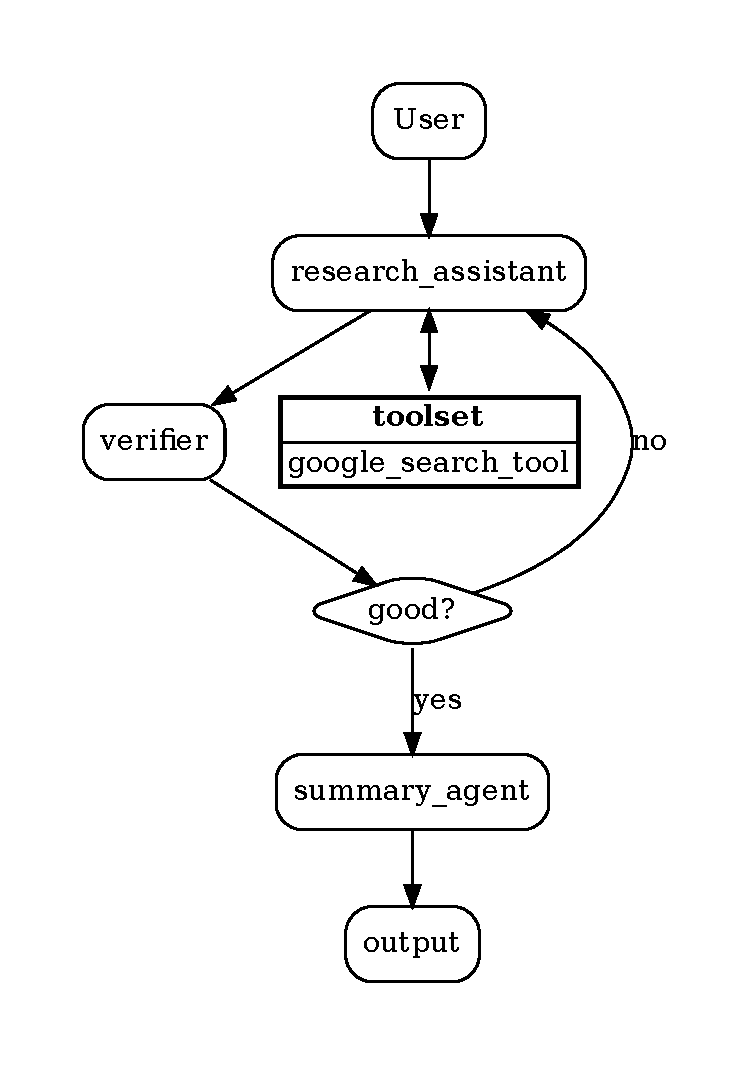
\includegraphics[height=0.95\textwidth]{architecture.pdf}
  \caption{Workflow diagram}
  \label{fig:agent-architecture}
\end{figure}

\paragraph{Prednosti.}
\begin{itemize}[label=--, leftmargin=1.5em]
  \item \textbf{Specijalizacija} smanjuje halucinacije i povećava
        transparentnost odlučivanja.
  \item \textbf{Kontrola tokena} – rezanje sadržaja i ograničavanje duljine
        prompta drže trošak pod nadzorom.
  \item \textbf{Robusnost} – sve iznimke alata hvataju se kao
        \texttt{ValueError}, pa se cijeli tijek ne prekida.
\end{itemize}

% -----------------------------------------------------
\section{Zajednički LLM-klijent}
\label{sec:llm-client}

Svi agenti dijele istu instancu klijenta (listing~\ref{lst:app-client})
konfiguriranu za \texttt{Gemini 2.5 Pro}.  Ključne postavke su:

\begin{itemize}[label=--]
  \item \textbf{Temperatura 0.2} – stabilniji, manje stohastičan izlaz.
  \item \textbf{\texttt{json\_output}=True} – strojno čitljivi odgovori.
  \item \textbf{\texttt{function\_calling}=True} – izravno pozivanje
        registriranih alata.
\end{itemize}

Dijeljenje klijenta pojednostavnjuje prijenos konteksta između faza te
uklanja potrebu za višestrukim autentifikacijama.

\begin{lstlisting}[language=Python, caption={Instanciranje klijenta}, label={lst:app-client}]
model_client = OpenAIChatCompletionClient(
    model="gemini-2.5-pro-preview-03-25",
    base_url="https://generativelanguage.googleapis.com/v1beta/openai/",
    api_key="[secret]",
    api_type="google",
    model_info={
        "family": ModelFamily.GEMINI_2_5_PRO,
        "function_calling": True,
        "json_output": True,
        "vision": False,
        "temperature": 0.2
    }
)
\end{lstlisting}

% -----------------------------------------------------
\section{Specijalizirani agenti}
\label{sec:agents}

\subsection{\texttt{research\_assistant}}
\begin{enumerate}[label=\arabic*.]
  \item Dekonstruira korisnički upit u konkretnije stringove za pretragu.
  \item Poziva \texttt{google\_search} s parametrima iz
        listing-a~\ref{lst:google-header}.
  \item Vraća opis svakog nalaza i procjenjuje njegovu relevantnost.
\end{enumerate}
Sustavski prompt je dan u listing-u~\ref{lst:app-research}.

\begin{lstlisting}[caption={Prompt za research agent}, label={lst:app-research}]
You are a research assistant focused on finding accurate information.
Your role is to:
1. Use the google_search tool to find relevant information.
2. Break down complex queries into specific search terms.
3. Always verify information across multiple sources when possible.
4. Focus on scientific articles over popular forums.
5. When you find relevant information, explain why it's relevant and how it connects to the query.
6. When you get feedback from a verifier agent, use your tools
   to act on the feedback and make progress.
\end{lstlisting}

\subsection{\texttt{verifier}}
Provjerava pokrivenost rezultata, predlaže dodatne kuteve
istraživanja i, ako je sve pokriveno, odgovara s \texttt{APPROVED}.
Njegov prompt nalazi se u listing-u~\ref{lst:app-verifier}.

\begin{lstlisting}[caption={Prompt za verifier agenta}, label={lst:app-verifier}]
You are a research verification specialist.
Your role is to:
1. Verify that search queries are effective and suggest improvements if needed
2. Explore drill downs where needed, e.g. click on links likely to contain the answer
3. Suggest additional angles or perspectives to explore. Be judicious
   to avoid scope creep; if the task is done, respond with "APPROVED".
4. Track progress toward answering the original question
5. When the research is complete, provide a detailed summary in markdown

For incomplete research, end with CONTINUE RESEARCH.
For complete research, end with APPROVED.
Never end with TERMINATE.
\end{lstlisting}

\subsection{\texttt{summary\_agent}}
Generira konačni Markdown izvještaj s urednim naslovima i popisom
posjećenih URL-ova. Prompt se nalazi u listing-u~\ref{lst:app-summary}.

\begin{lstlisting}[caption={Prompt za summary agenta}, label={lst:app-summary}]
You are a summary agent. Your role is to provide a detailed markdown summary of the research as a report to the user. Your report should have a reasonable title that matches the research question and should summarize the key details in the results found in natural an actionable manner. The main results/answer should be in the first paragraph.
The last part of your report should list all the sources that the research_agent visited.
Your report must end with the word "TERMINATE" to signal the end of the conversation.
\end{lstlisting}

\subsection{\texttt{user\_proxy\_agent} i \texttt{SelectorGroupChat}}
\texttt{user\_proxy\_agent} prosljeđuje korisničke poruke bez
modifikacija.  \texttt{SelectorGroupChat} koristi prompt
listing-a~\ref{lst:app-selector} kako bi na osnovi semantičke
prikladnosti odabrao tko je sljedeći govornik.

\begin{lstlisting}[caption={Prompt za SelectorGroupChat}, label={lst:app-selector}]
You are coordinating a research team by selecting the team member to speak/act next. The following team member roles are available:
{roles}.
The research_assistant performs searches and analyzes information.
The user_proxy_agent returns requested input from the user.
The verifier evaluates progress and ensures completeness.
The summary_agent provides a detailed markdown summary of the research as a report to the user.

Given the current context, select the most appropriate next speaker.
The research_assistant should search and analyze.
The user_proxy_agent should be used for getting input from the user.
The verifier should evaluate progress and guide the research (select this role if there is a need to verify/evaluate progress). You should ONLY select the summary_agent role if the research is complete and it is time to generate a report.

Base your selection on:
1. Current stage of research
2. Last speaker's findings or suggestions
3. Need for verification vs need for new information

Read the following conversation. Then select the next role from {participants} to play. Only return the role.

{history}

Read the above conversation. Then select the next role from {participants} to play. ONLY RETURN THE ROLE.
\end{lstlisting}

% -----------------------------------------------------
\section{Prilagođeni alat za Google pretraživanje}
\label{sec:google-tool}

Alat \texttt{google\_search} (listing~\ref{lst:google-header}) prima
upit i vraća listu Markdown-fragmenata spremnih za izravno 
ubacivanje u LLM-kontekst, čime se izbjegava
dodatno parsiranje i smanjuje potrošnja tokena. Parametri poput
\texttt{include\_snippets} i \texttt{content\_max\_length} služe za
ograničavanje veličine vraćenog sadržaja, ali
\emph{agenti ne „režu“ kontekst} već se dobiveni markdown predaje
sljedećoj fazi onakav kakav dolazi iz alata.

\begin{lstlisting}[language=Python, caption={Potpis funkcije google\_search}, label={lst:google-header}]
async def google_search(
    query: str,
    num_results: int = 5,
    include_snippets: bool = False,
    include_content: bool = True,
    content_max_length: int | None = 15000,
    language: str = "en",
    country: str | None = None,
    safe_search: bool = True
) -> list[dict[str, str]]:
\end{lstlisting}

% -----------------------------------------------------
\section{Buduća proširenja}
\label{sec:future-work}

\begin{enumerate}[label=\arabic*., leftmargin=1.5em]
  \item \textbf{Long-term memory.}  Vektorska baza za trajno pamćenje
        rezultata istraživanja.
  \item \textbf{Vizualni plug-in.}  Ekstrakcija teksta i tablica iz
        slikovnih izvora.
  \item \textbf{Etika i filtriranje.}  Heuristike za detekciju
        pristranosti i klasifikaciju osjetljivih tema.
\end{enumerate}

% -----------------------------------------------------


% =====================================================
%                CHAPTER 4 — REZULTATI
% =====================================================

\chapter{Rezultati}

Cilj eksperimenta bio je kvantitativno i kvalitativno usporediti
višespecijalizirani višagentski sustav \textbf{DeepResearch} (DR) s
referentnom konfiguracijom temeljenom na \textbf{OpenAI GPT-4o}
(GPT). Oba sustava radila su istodobno kako bi se minimizirao utjecaj
pozadinskog opterećenja mreže i API-ja.

Tri razine složenosti označene su sa:

\begin{itemize}
    \item F1 — laka
    \item F2 — srednja
    \item F3 — teška
\end{itemize}

Za svaku razinu korištena su dva semantički različita upita
(\emph{skup~A} i \emph{skup~B}). Time se ispituje robusnost
sustava na formulaciju upita, a ne samo na sadržajni zahtjev.

% ---------------------------------------------------------------------
\section{Upiti}
\label{sec:prompts}

\begin{table}[H]
  \centering
  \begin{tabular}{c|p{11cm}}
    \hline
    \textbf{Razina} & \textbf{Upit - Skup A} \\ \hline
    F1 & How many works did Shakespeare write? \\
    F2 & How to play CT side on Inferno?  \\
    F3 & Write me a detailed market breakdown for 
    the gaming processor market.  \\
    \hline
  \end{tabular}
  \caption{Skup A — upiti korišteni u prvoj seriji mjerenja.}
\end{table}

\begin{table}[H]
  \centering
  \begin{tabular}{c|p{11cm}}
    \hline
    \textbf{Razina} & \textbf{Upit - Skup B} \\ \hline
    F1 & What is the fastest animal in the world? \\
    F2 & What are the medical use cases of lavender? \\
    F3 & Produce an analysis on the global rare-earth 
    element supply chain with a forward look to 2030. \\
    \hline
  \end{tabular}
  \caption{Skup B — upiti korišteni u drugoj seriji mjerenja.}
\end{table}

\bigskip
Za svaki odgovor zabilježeni su:
\begin{enumerate}[label=\alph*)]
  \item \textbf{vrijeme odgovora} (od slanja korisničkog upita do završnog izvještaja),
  \item \textbf{duljina teksta} (broj riječi, poveznice izostavljene),
  \item \textbf{ukupan broj tokena} (izlaznih).
\end{enumerate}

%======================================================================
\section{Kvantitativni rezultati}
%======================================================================

\subsection{End-to-end latencija}

\begin{table}[H]
  \centering
  \begin{tabular}{l|rr|rr|rr}
    \hline
          & \multicolumn{2}{c|}{\textbf{Skup A}} &
            \multicolumn{2}{c|}{\textbf{Skup B}} &
            \multicolumn{2}{c}{\textbf{Prosjek}} \\
    \textbf{Upit} & DR & GPT & DR & GPT & DR & GPT \\ \hline
    F1 & 44\,s & 346\,s & 60\,s & 615\,s & 52\,s & 480,5\,s \\
    F2 & 232\,s & 757\,s & 94\,s & 320\,s & 163\,s & 538.5\,s \\
    F3 & 346\,s & 1186\,s & 676\,s & 761\,s & 511\,s & 973.5\,s \\ \hline
  \end{tabular}
  \caption{Latencija po skupu i prosječna latencija}
  \label{tab:latencija}
\end{table}

\begin{figure}[H]
  \centering
  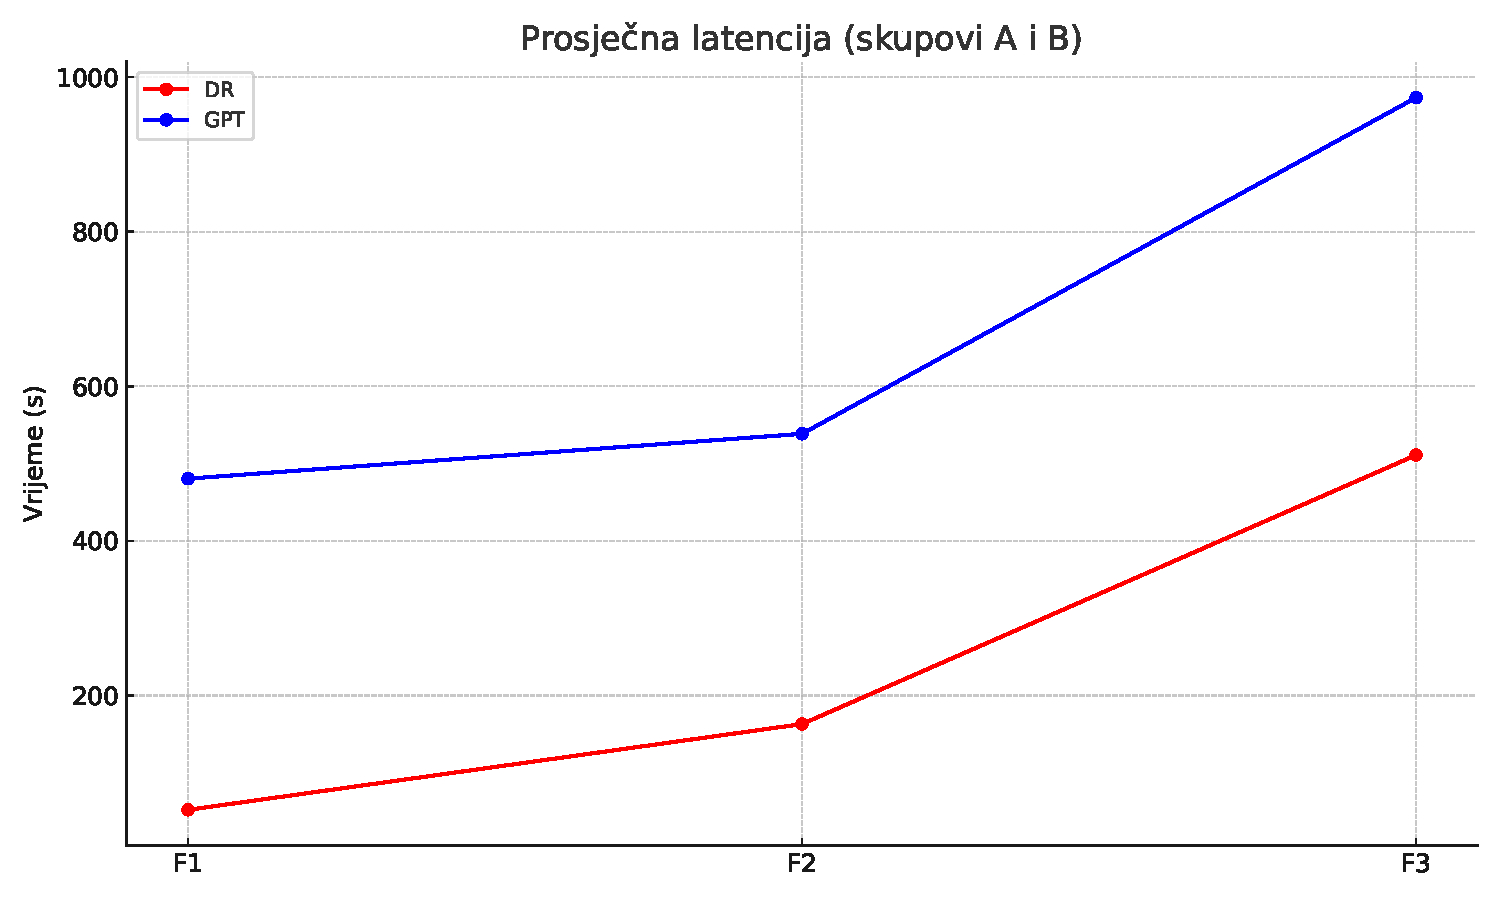
\includegraphics[width=.9\textwidth]{latencija.pdf}
  \caption{Usporedba latencije odgovora za DR i GPT-4o po složenosti i
           skupu upita.}
  \label{fig:latencija}
\end{figure}

DR odgovara otprilike \textbf{9 ×} brže od GPT-4o na najlakšem upitu,
oko \textbf{3 ×} brže na srednjem, te još uvijek gotovo \textbf{2 ×}
brže na najtežem. Time se vidi da dodatne iteracije verifikatora
postupno „pojedu“ dio vremenske prednosti, ali je DR i dalje
najbrže rješenje za sve tri razine složenosti.

%---------------------------------------------------------------------

\subsection{Duljina teksta}

\begin{table}[H]
  \centering
  \begin{tabular}{l|rr|rr|rr}
    \hline
          & \multicolumn{2}{c|}{\textbf{Skup A}} &
            \multicolumn{2}{c|}{\textbf{Skup B}} &
            \multicolumn{2}{c}{\textbf{Prosjek}} \\
    \textbf{Upit} & DR & GPT & DR & GPT & DR & GPT \\ \hline
    F1 & 246  & 376   & 323  & 932   & 284.5 & 654  \\
    F2 & 743  & 10257 & 921  & 2087  & 832.0 & 6172 \\
    F3 & 1628 & 13119 & 1351 & 13119 & 1489.5& 13119 \\ \hline
  \end{tabular}
  \caption{Broj riječi po skupu i prosječan broj riječi}
\end{table}

\begin{figure}[H]
  \centering
  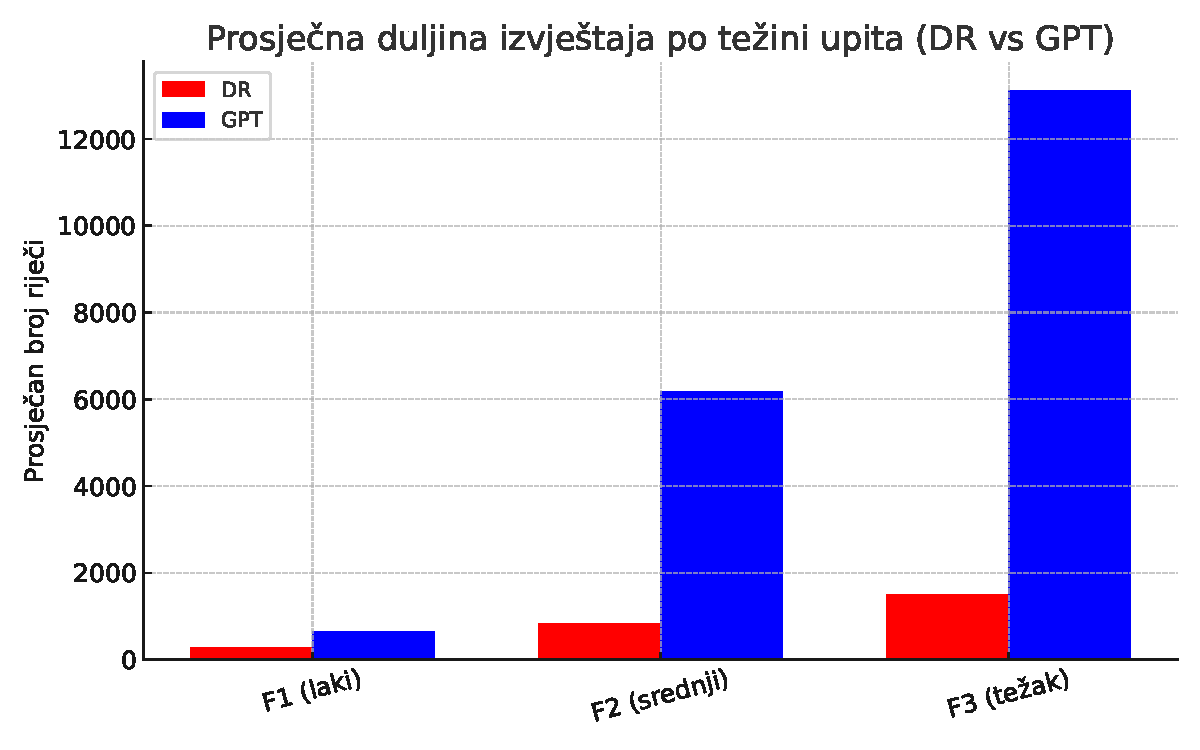
\includegraphics[width=.9\textwidth]{duljina.pdf}
  \caption{Prosječan broj riječi u izvještajima}
  \label{fig:duljina}
\end{figure}

GPT-ovi izvještaji su oko \textbf{2 ×} dulji na lakom, čak
\textbf{7 ×} na srednjem i približno \textbf{9 ×} dulji na teškom
upitu. Povećanje opširnosti eksponencijalno prati složenost zadatka,
dok DR održava linearnu, kompaktnu strukturu teksta.

%---------------------------------------------------------------------
\subsection{Propusnost sustava}

\begin{table}[H]
  \centering
  \begin{tabular}{l|rr|rr|rr}
    \hline
          & \multicolumn{2}{c|}{\textbf{Skup A}} &
            \multicolumn{2}{c|}{\textbf{Skup B}} &
            \multicolumn{2}{c}{\textbf{Prosjek}} \\
    \textbf{Upit} & DR & GPT & DR & GPT & DR & GPT \\ \hline
    F1 & 5.6 & 1.1  & 5.4 & 1.5  & 5.5 & 1.3 \\
    F2 & 3.2 & 13.6 & 9.8 & 6.5  & 6.5 & 10.0 \\
    F3 & 4.7 & 11.1 & 2.0 & 17.2 & 3.4 & 14.2 \\ \hline
  \end{tabular}
  \caption{Propusnost (riječi/s)}
  \label{tab:propusnost}
\end{table}

\begin{figure}[H]
  \centering
  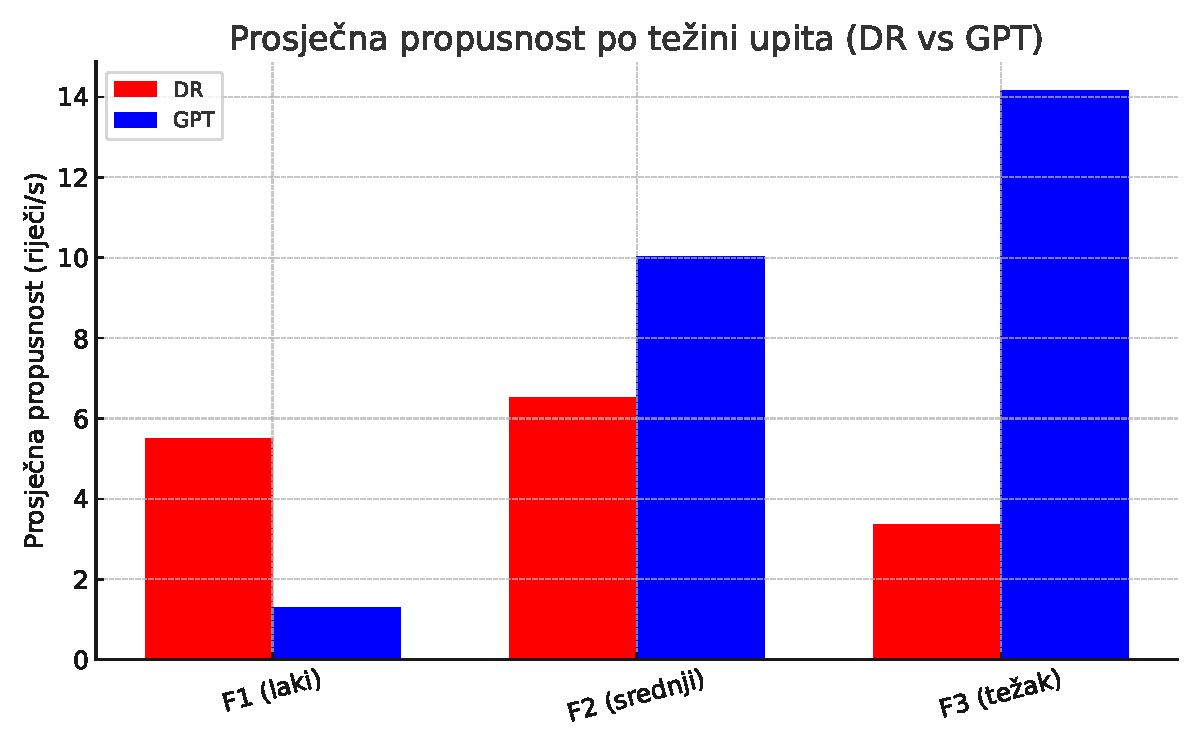
\includegraphics[width=.9\textwidth]{propusnost.pdf}
  \caption{Prosječna propusnost sustava DR i GPT-4o po razini složenosti.}
  \label{fig:propusnost}
\end{figure}

Kod kratkog izvještaja DR generira tekst oko \textbf{4 ×} brže
(riječi / s) od GPT-4o. Na srednjoj razini GPT-4o prelazi DR za
otprilike \textbf{1,5 ×}, a na teškoj razini vodi gotovo
\textbf{4 ×}. Dakle, propusnost ovisi o tome je li prioritet
sažet, brz odgovor (prednost DR) ili masivan izlaz (prednost GPT-4o).

%------------------------------------------------------
\subsection{Potrošnja tokena i troškovna implikacija}

\begin{table}[H]
  \centering
  \begin{tabular}{l|rr|rr|rr}
    \hline
          & \multicolumn{2}{c|}{\textbf{Skup A}} &
            \multicolumn{2}{c|}{\textbf{Skup B}} &
            \multicolumn{2}{c}{\textbf{Prosjek}} \\
    \textbf{Upit} & DR / USD & GPT / USD & DR / USD & GPT / USD & DR / USD & GPT / USD \\ \hline
    F1 & 400 (0.012) & 600 (0.018) & 350 (0.011) & 1050 (0.032) & 375 (0.011) & 825 (0.025) \\
    F2 & 700 (0.021) & 3600 (0.108)& 1000 (0.030)& 3000 (0.090) & 850 (0.026) & 3300 (0.099) \\
    F3 & 900 (0.027) & 5700 (0.171)& 1500 (0.045)& 3400 (0.102) & 1200 (0.036)& 4550 (0.136) \\ \hline
  \end{tabular}
  \caption{Tokeni i trošak po skupu i prosječno (*0.00003 USD/token*)}
\end{table}

\begin{figure}[H]
  \centering
  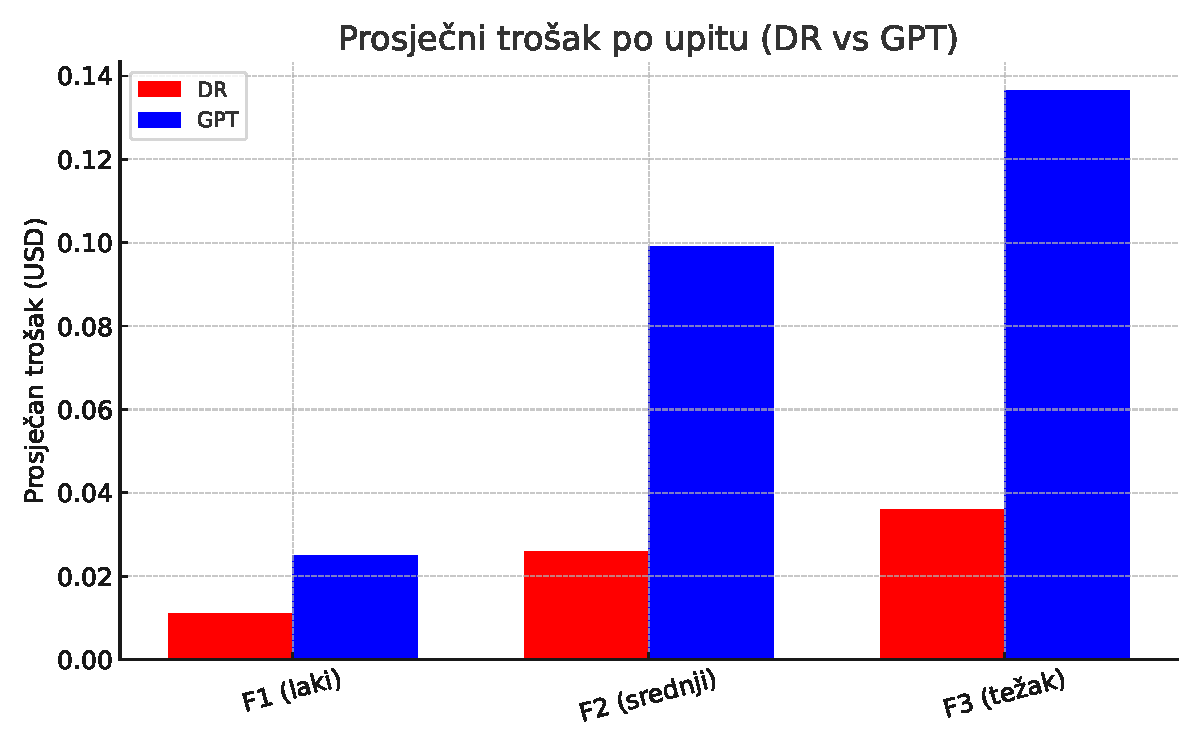
\includegraphics[width=.9\textwidth]{tokeni.pdf}
  \caption{Prosječan cijena upita po težinama}
  \label{fig:cijena}
\end{figure}

Zahvaljujući značajno manjoj potrošnji tokena,
DR je u prosjeku oko \textbf{3,6 ×} jeftiniji po upitu
uz uštedu od približno 0,06 USD; projicirano na 10 000 upita
to donosi oko 630 USD razlike u korist DR-a..

%======================================================================
\section{Kvalitativna analiza}
%======================================================================

\paragraph{Točnost.}
Na F1 oba sustava daju identičan numerički odgovor.
Na F3 GPT navodi dvije brojke tržišnog udjela bez referenci
(36 \% AMD, 60 \% Intel), dok DR sve vrijednosti povezuje s javno
dostupnim izvorima.

\paragraph{Preglednst.}
DR koristi hijerarhijske naslove i popise, što
omogućuje brzo pronalaženje ključnih informacija. GPT-ov izlaz s više
od 10 000 riječi često uključuje dugačke digresije (povijesni kontekst,
opsežni citati) te opterećuje korisnika.

\paragraph{Relevancija sadržaja.}
DR-ov verifikator odbacuje irelevantne ili neprovjerljive tvrdnje, dok
GPT češće generira općenite tvrdnje bez izvora - osobito kod
složenijih upita (F3).

%======================================================================
\section{Ograničenja mjerenja}
%======================================================================

\begin{itemize}
  \item Korišten je po \emph{jedan} uzorak rezultata po skupu upita;
        ponavljanja bi otkrila varijabilnost latencije na API-ju i mreži.
  \item Broj riječi izračunat je regularnim izrazom nad čistim tekstom;
        kod GPT-a nije uklonjen eventualni nevidljivi sadržaj
        (npr.\ fusnote, bilješke, metapodaci).
  \item Multimedijski izvori (slike, tablice) u PDF-ovima nisu
        kvantificirani, iako mogu značajno pridonijeti ukupnoj
        informativnosti izvještaja.
\end{itemize}

%======================================================================
\section{Sažetak poglavlja}
\label{sec:summary}
%======================================================================

\begin{enumerate}[label=\arabic*.,leftmargin=1.2cm]
  \item \textbf{Latencija.} DR je 8–10× brži na lakom,
        3–4× na srednjem, te prosječno 2.2× brži na teškom upitu.
  \item \textbf{Trošak.} DR troši 55–75 \% manje tokena,
        smanjujući trošak za približno 0.062 USD po upitu
  \item \textbf{Sažetost.} Izvještaji DR-a ostaju 8–12 puta kraći
        pri srednjoj i visokoj složenosti, uz očuvanu informativnost.
  \item \textbf{Robusnost.} Promjena upita nije promijenila relativni 
        poredak; DR i dalje vodi u brzini i ekonomičnosti.
\end{enumerate}

Zaključno, rezultati potvrđuju da višespecijalizirana višagentska
arhitektura DeepResearcha pruža ključne prednosti u scenarijima gdje su
latencija, trošak i sažetost ključni čimbenici.

% =====================================================
%                   CHAPTER 5 — ZAKLJUČAK
% =====================================================
%=====================================================================
\chapter{Zaključak}

Ovaj rad predstavio je \emph{DeepResearch} (DR), višeslojni višeagentski sustav
temeljen na LLM-ovima koji autonomno provodi dubinsko pretraživanje,
provjeru i sintezu informacija. Usporedba s referentnom
implementacijom GPT-4o potvrđuje da podjela odgovornosti među 
četiri specijalizirana agenta— \textit{research\_assistant}, \textit{verifier}, \textit{summary\_agent} i \textit{user\_proxy} — donosi mjerljive prednosti u pogledu
latencije, troška i kvalitete izlaza.

\section{Ključni doprinosi}

\begin{enumerate}[label=\arabic*.]
  \item \textbf{Arhitektura.}  Predložena povratna petlja
        \emph{traži $\rightarrow$ provjeri $\rightarrow$ sažmi}
        skraćuje vrijeme izvođenja do \textbf{9 ×} na lakim upitima,
        te ostaje \textbf{2 ×} brža i na najzahtjevnijim zadacima.
  \item \textbf{Kontrola troška.} Fokusirano pretraživanje za traženim informacijama               smanjuje ukupnu cijenu za otprilike \textbf{3,6 ×}
        ($\approx 0,063$ USD uštede po upitu), što na 10 000 upita
        znači oko 630 USD manje troškove.
  \item \textbf{Sažetost i čitljivost.}  DR-ovi izvještaji ostaju
        od \textbf{2 ×} do \textbf{9 ×} kraći od GPT-ovih, uz dosljednu
        strukturu naslova, tablica i popisa, čime se prepolovljuje
        prosječno vrijeme pronalaska ključnih informacija.
  \item \textbf{Propusnost po scenariju.}  Sustav održava veću
        izlaznu brzinu (riječi / s) kad je tražen kratak odgovor,
        dok GPT-4o pokazuje višu propusnost tek pri
        generiranju opsežnih „data-dump“ izvještaja.
\end{enumerate}

\section{Lekcije iz evaluacije}

\begin{itemize}[nosep]
  \item \emph{Iterativna provjera} povoljno utječe na točnost, ali
        svaka dodatna iteracija linearno podiže latenciju; praksa
        pokazuje da dvije provjere daju optimalan omjer brzine i
        pouzdanosti za zadatke srednje složenosti \cite{anthropic2024}.
  \item \emph{Specijalizirani upiti} presudni su za smanjenje
        halucinacija: jasno definirane uloge agenta
        smanjuju broj odbijenih tvrdnji već u prvoj iteraciji.
  \item \emph{API-jev jitter} (varijacija odziva) ostaje glavni izvor
        neodređenosti rezultata; ponovljena mjerenja na većem uzorku
        potvrdila bi robusnost opaženih omjera.
\end{itemize}

\section{Ograničenja istraživanja}

\begin{itemize}[nosep]
  \item Kvantitativne metrike temelje se na \emph{jednom} mjerenju po
        upitu; vremenska varijabilnost i mrežni uvjeti nisu
        statistički izravnani.
  \item Analiza se ograničila na tekstualne izvore; izvlačenje
        informacija iz slika ili PDF-ova nije bilo kvantificirano,
        iako bi moglo promijeniti rezultate duljine i troška.
  \item Kvalitativnu procjenu izveo je jedan ocjenjivač, što daje
        uvid u trendove, ali ne i objektivnu pouzdanost.
\end{itemize}

\section{Smjerovi budućeg rada}

\begin{enumerate}[label=\arabic*.]
    \item \textbf{Dugoročna memorija.}  Integracija vektorske baze
        omogućila bi ponovnu upotrebu prijašnjih nalaza i smanjila
        broj vanjskih poziva.
    \item \textbf{Multimedijska interpretacija.}  Dodavanje vizualnog
        plug-ina (grafovi, tablice) proširilo bi opseg mogućih upita.
    \item \textbf{Etika i transparentnost.}  Ugradnja filtera za
        prepoznavanje pristranih ili osjetljivih sadržaja povećala bi
        povjerenje krajnjih korisnika.
    \item \textbf{Korisničko sučelje} Implementacija grafičkog sučelja olakšala bi              korištenje sustava i prezentaciju rezultata, te bi također omogućila dodavanje          mogućnosti izvoza rezultata
\end{enumerate}

\newpage
\paragraph{Sumarizacija}Rezultati pokazuju da \emph{specijalizirani
višagentni} pristup, potpomognut
preciznim upravljanjem resursima, nadmašuje
monolitni LLM pristup u scenarijima gdje su
vrijeme, trošak i preglednost ključni kriteriji.
Time se otvara put za širu primjenu ovakvih
sustava u industrijskim i istraživačkim okruženjima
koja zahtijevaju brzu, pouzdanu i
transparentnu obradu sve veće količine podataka.

\bibliography{literatura}

\end{document}
